\section{Education and Training}
\label{sec:education}
\subsection{\bf About the ACMS program}

The ACMS {\em (Applied and Computational Mathematical Sciences)} was
introduced in 1998 as a joint undergraduate program between the
departments of Applied Mathematics, Computer Science and Engineering
(CSE), Mathematics, and Statistics, among others.

The ACMS program is structured into a {\em core} set of courses,
totaling 43 credits, and a set of options, or {\em tracks}. The tracks
are either associated with a particular application domain (Biological
and Life Sciences, Mathematical Economics, Social and Behavioral
Sciences, Engineering and Physical Sciences) or with a particular area
of specialization in the mathematical sciences ({\em Discrete Math and
  Algorithms, Operations Research, Scientific Computing and Numerical
  Analysis, and \underline{Statistics}}).

It is the Statistics track of ACMS that we are aiming to
tranform. Currently, this track contains, in addition to the core
courses, the following:
\\
{\bf Option Core (37 credits)}
\bits
    \item {\sc PHYS 121-2-3} (replaceable by other courses in application areas)
    \item {\sc STAT 302} Statistical Software and Its Applications (R course, irregularly offered, 2 credits)
    \item {\sc STAT 340} Probability and Mathematical Statistics
    \item {\sc STAT 341-2} to Probability and Statistical Inference I,II
    \item {\sc STAT 421} Applied Statistics and Experiment Design
    \item {\sc STAT 423} Applied Regression and Analysis of Variance
\eits
{\bf Option Electives (10 credits)}
\bits
    \item {\sc MATH/STAT 396} Probability III
    \item {\sc MATH/STAT 491-2} Stochastic Processes
    \item {\sc STAT 403}  Resampling Inference
    \item {\sc STAT 427}  Analysis of Categorical Data
    \item {\sc STAT/BIOST 529} Sample Survey Techniques
    \item {\sc CSE 373} Data Structures
    \item {\sc MATH 300} Mathematical Reasoning
    \item {\sc MATH 327}  Real Analysis I
    \item {\sc MATH 407--8--9} Linear, Nonlinear,\& Discrete Optimization
    \item {\sc STAT 428} Multivariate Analysis for the Social Sciences
    \item {\sc GEOG 426} Quantitative Methods in Geography
    \item {\sc QMETH 528} Survey Sampling Applications
    \item {\sc STAT 498} Special topics
\eits
The program web page recommends that ``[this track] is ideally suited as a {\em second major} for students with a primary focus in the [\ldots] sciences''.
De facto, the track curriculum differs little, most notably by the
presence of the computer programming class {\sc CSE 142}, from the
``standard'' Statistics major.

{\bf Enrollment} The ACMS major is competitive, with the number of
majors capped at about 200.  During the recent academic years,
graduation numbers have passed 100 students per year; the current
enrollment is at 147\footnote{Complete breakdown of ACMS graduation
  numbers from 1998 on are in the Supplementary material.}.  Of these,
the Statistics track accounts for 4 students currently enrolled (none
as double majors), and for 2 to 6 students graduated in each of the
last 5 years. In the same time, enrollment in the Statistics major is
at an all times high, with \mmp{fill} of which XX women.

\subsection{Transforming the Statistics  ACMS track}
We will transform the ACMS Statistics track into a virtually new
major, a ``computationally minded Statistics major focused on Big Data''. 
In other words, we will not aim to produce scientists who also know statistics (which
can be well served by Statistics minor and other tracks of ACMS) but
full-fledged statisticians who can function autonomously in the modern
cyberworld.

There are several motivating factors:
\bit
\item Interest in statistics is at an all times high, as witnessed by
  our enrollment numbers. We expect that the ACMS Statistics track
  will reach similar enrollment numbers. Note that at the current
  enrollment in the other tracks, the total ACMS enrollment will be
  near the 200 level.

\item The role of
  the statistician as data analyst has become both more central, and
  more demanding. As more data analysis and more decisions based on it
  are being shifted from humans to computers, statistics is called
  upon to design and validate the procedures used to take these
  decisions. Thus, the statician's importance in a much wider range of
  human activities, be they science or business. But the
  statistician's responsibility is commensurately growing, as (s)he needs
  to master the skills required by cyber-enabled science and data
  analysis.
\item These skills are not limited to using computers and
  programming. The nature of statistical analyses itself is
  affected \mmp{get some citations} as it has been long
  recognized. Computationally heavy statistical methods need to be
  designed. Very large samples will support models of a complexity
  that could not be considered in real-life scenarios a decade or two
  ago. It is now not possible to perform model selection by explicitly
  comparing all possible models (i.e. there can be an exponential
  number of models to compare) and regularization methods are often
  called into play, as are approximate computational
  techniques. Leveraging unlabeled data for prediction is now an
  almost universal necessity. Devising new methods to evaluate complex
  models in an environment that is not stationary, nor controlled are
  some of the challenges of modern data analysis.
\item The proposal fits in and leverages other \cdse\ efforts and successes at UW in creating a strong collaborative environment for (the e-science Institute, the IGERT for graduate education in Big Data and the related PhD tracks recently created in CSE and Statistics). The time is ripe to involve undergraduates, and specifically statistics and mathematics majors in this change.
\item This proposal is in the spirit of the ACMS original mission,
  bringing this part up to speed with the demands of the coming decade.
\eit

{\bf Work Plan}

For planning purposes, we divide the proposed project into three stages which
roughly map to yearly schedule. 

{\bf Stage 1:} Design and introduce two new courses \statcl, \astrocl,
as {\em electives} in the track.  Start the Undergraduate \cdse~
Research Seminar. This seminar will differ from the existing ``ACMS''
Undergraduate Math Science Seminar ({\sc Math 498}), in that the
speakers will be undergraduates themselves or their mentors, and the
seminar topics will be their projects (see Section
\ref{sec:ugrad-seminar} for more details).

{\bf Stage 2:} Redesign the track: move \statcl, Stochastic Processes {\sc STAT 481, 482} into the core. As the track will no longer be regarded as a second major for science students, we will make room by removing the {\sc PHYS 121-2-3} courses (15 credits) from it.  Reorganizing the electives into two groups: math/stat electives (group I) and computing and science electives (group II). Further reorganization of the core and electives in consultation with Statistics faculty and the other ACMS participating departments and Schools. For example, we will consider adding one or both of {\sc AMATH 482, 483} ``Data analysis'', ``High performance scientific computing''.

Organization of a workshop for UW faculty to share our experiences and teaching infrastructure.

{\bf Stage 3:} Incorporate feedback from evaluators and all participants. Continue developing the courses' software and data infrastructure. 

In addition to this plan, although we are at the moment not explicitly
proposing this, we will investigate if the two new courses could be
made accessible to Mathematics majors as well. Mathematics Professor
William Stein, creator and leader of the {\tt Sage} project, teaches a
successful Python programming course in Mathematics, which could serve
to build a pathway towards one or both of the two new courses, if a
way to satisfy the Statistics prerequisites is also found.


{\bf Why this particular approach?} Currently, computer education is
assured primarily through two core courses, {\sc CSE 142, 143}
\cite{cse142}. These set the foundations in the understanding of
computer programming, but they are of a general nature, and are mainly
focused towards preparing future programmers  (these courses are the
same courses that the approximately 500 CSE majors take). Thus, there
is no room for data analysis applications in these courses.  There is
also a programming in R course ({\sc STAT 302}, 2 credits) but it is 
offered quite irregularly.

However, for reasons we will expound later (Section \ref{sec:Python}), we
consider that Python is the more appropriate computer language for our
goals. Thus, we will both introduce Python and will use it to teach
statistical methodology.  As Python will be taught as a second
programming language, and as it is similar enough to Java (taught in
CSE 142), we expect the students to assimilate it quickly under our
guidance (there are also numerous publicly available tutorials).
In Spring 2013, a pilot course was taught (by H. Koepke,
Statistics) that introduced Python and taught statistical modeling
using the language, to an audience of around 40 CSE undergraduates
(the vast majority of wich did {\em not} know Python). The students'
feedback was very encouraging, and one of the reasons we are confident
in our approach.

The need for a dedicated scientific computing course was long
recognized, hence the Scientific Computing track and courses developed
by AMATH {\sc 481} (project based, in Matlab) {\sc 482}, and {\sc 483}. 
Our proposed courses are not replicating, but adding a new dimension to
the existing AMATH courses. The latter focus on the ``signal
processing'' aspects of data analysis (e.g filtering, {\sc AMATH
  482}) and on the ``hardware, software, and programming for
large-scale scientific computing'' ({\sc AMATH 483}), while our
courses focus on the statistical modeling and statistical decision
making aspects.
 
\comment{

next steps: other math majors?, new certificates, programs

MMP -find out about minors

will also help students in hard/soft sciences 


\section{University involvement}

UW context: e-sci, igert, phd tracks in stat, cse,..., 
stat context: increased interest in stats/data sci Statistics is recognized (by students themselves) at the forefront of the data science revolution. Phd track, MS track.

Astro involvement

How does UW support this plan:



}%end comment

\subsection{Description of the courses}
\label{sec:course-descr}

\bits
\item \statcl 
``Computational Statistical Modeling and Machine Learning'' (4 credits)
\item \astrocl ``Data Intensive Astronomy'' (3 credits)
\eits
These courses' aims are explicitly to (1) to give students a hands-on experience, through programming, and performing real data analyses on a computer, with the computational aspects of 
statistical modeling in general, and (2) to introduce them to the  machine learning methodology in particular, with specific attention to the issues of big data.

The material covered will be partly overlapping with other courses
(e.g. regression, probability models for discrete data) and partly new
(e.g. classification, clustering). However, the treatment of the
material will stress on the interaction of computational and
statistical aspects in modeling and prediction with scientific and
engineering data. In this sense, the overlap has not been avoided on purpose
so that the students can gain a new, computational, perspective on areas
already studied from a more theoretical point of view. 

{\bf Prerequisites} (for either course): an introductory programming
course (not necessarily in Python), e.g. CSE 142 or equivalent
programming experience; an introductory statistics course; mathematics
multivariate calculus. The two courses can be taken in a sequence
\statcl--\astrocl, or separately. These course can be accessible to
other juniors and seniors with a strong quantitative background.

\bit
\item  \underline{\statcl~ Draft Syllabus}\\
  - a review of the concept of likelihood and Max Likelihood estimation (cases in which MLE has no closed form, gradient ascent/Newton estimation of MLE)\\
  - a review of basic probability models with focus on ML estimation of these models, supported heavily by simulation (e.g demonstrating gaussianity of MLE for certain models, and non-gaussianity for other models, including Zipf's law type distributions)\\
  - models for statistical prediction, with focus on classification\\
  - review and computational aspects of other statistical topics like
  density estimation, clustering, model selection and validation
  (including regularization and  nonparametric modeling)\\
  - intro to programming in Python, and to Python libraries supporting scientific computing\\
  - examples of real applications from engineering and sciences (image
  analysis, information retrieval, etc.)

\item[]{\bf Learning goals for \statcl} Ability to perform computationally intensive, automated, robust and efficient data analysis. Ability to combine existing tools and libraries with programming in a general purpose language (Python). 
Working knowledge of the most important/main machine learning tools and methods, as well as their probabilistic interpretation. Understanding of the practical implications of theoretical results like independence, overfitting, consistency of an estimator. 

{\bf Textbooks} Unfortunately, there is no single textbook one can
assign for this course. We will rely partly on \meila's previously
developed course notes for {\it ``Probability and Statistics for
  Computer Science''}, a computationally minded introductory course,
partly on new course notes to be developed by \meila\ specifically for
this more advanced course, and partly on the textbook of \astrocl, 
which will provide among others the Python exercises. We are also
considering a new machine learning book written for undergraduate
students \cite{x}. 

\comment{
\item{Motivation for \astrocl} \mmp{shorter,more to the point of grant}
Astronomy and astrophysics are witnessing dramatic increases in data volume 
as detectors, telescopes, and computers become ever more powerful. During the 
last decade, sky surveys across the electromagnetic spectrum have collected 
hundreds of terabytes of astronomical data for hundreds of millions of sources. 
Over the next decade, the data volume will enter the petabyte domain, and provide 
accurate measurements for billions of sources. Astronomy and physics students 
are not traditionally trained to handle such voluminous and complex data sets. 
Furthermore, standard analysis methods employed in astronomy often lag far 
behind rapid progress in statistics and computer science. The main
goal of this course is to contribute to efficient training of next
generations of students to 
handle the fast growing data sets, not only in astronomy, but in other quantitative 
sciences as well. 

This course will be aimed at physical and data-centric math,
statistics, science and engineering students
who have an understanding of the science drivers for analyzing large data sets but 
may not be aware of appropriate statistical techniques for doing so. The course work 
will provide to students a connection between scientific data analysis problems and 
modern statistical methods. We will limit theoretical discussions to the minimum 
required to understand the algorithms and will build the courses upon an 
example-driven compendium of modern statistical and data mining methods, 
together with carefully chosen examples based on real modern data sets, and of 
current astronomical applications that will illustrate each method introduced in the 
book. Discussion of the advanced material will be supported by appropriate (publicly 
available) Python code and data which will enable students to perform exercises, 
evaluate the techniques, and adapt them to their own fields of interest. We chose to 
use Python, a powerful and flexible programming language that is quickly becoming 
a standard in data-intensive sciences (and elsewhere). 

The target audience for our course includes undergraduate students
with scientific or engineering background, but it is likely that
graduate students would benefit from it too. Familiarity with calculus
and other basic mathematical techniques will be assumed, but no
extensive prior knowledge in statistics will be required.
}

\item \underline{\astrocl~ Draft Syllabus}\\

Computational Challenges in data-intensive astronomy and astrophysics: \\
- data types and data management systems \\
- types of computational problems and strategies for speeding them up \\
- data visualization challenges \\
- selection effects and truncated/censored data in astronomical context \\

Exploratory techniques and searching for structure \\
- non-parametric density estimation \\
- cluster finding methods (focus on non-parametrics and large data) \\

Dimensionality reduction\\
- review of principal component analysis in a large data context \\
- non-negative matrix factorization  \\
- independent component analysis and projection pursuit \\

Regression and model fitting for large data \\
- applications using real data from large sky surveys \\

Basics of time series analysis \\
- applications using real data from large sky surveys \\

Adoption and development of cross-disciplinary tools (e.g. numerical 
algorithms, visualization methods, data-human interaction) in the context
of big data, astronomical or otherwise (see Section \ref{sec:Python}).
\eit

{\bf Learning goals for \astrocl} \\
- familiarity with drivers for and accomplishments of modern astronomical surveys\\
- ability to perform computationally intense/automated and efficient data analysis\\
- ability to combine existing tools and libraries with programming in a general purpose language (Python)\\
- working knowledge of the most important/main machine learning tools and \\
   methods, as well as their probabilistic interpretation \\
- help to develop a diverse STEM workforce \\
 


{\bf Textbook} {\it ``Statistics, Data Mining, and Machine Learning in
  Astronomy: A Practical Python Guide for the Analysis of Survey
  Data''} (Princeton Series in Modern Observational Astronomy),  
coauthored by the Co-PIs on this proposal.

{\bf Format and student experience} 
The courses will consist of lectures, homework assignments, 1--2
miniprojects, and a final exam. The TA will hold quiz sections; about
half of these will be in a (virtual) computer lab environment. 

{\bf The Computer Lab recitations} will offer support for learning
Python, as well as specific data analysis tools (see Section \ref{sec:Python}).
The students will practice programming in pairs (a.k.a extreme
programming), using debuggers, profilers, writing modifiable code, etc.

Another experience in the computer lab will be actual data analysis
and visualization using the tools, the skills related to data
visualisation, experimental data recording and reporting, etc.

{\bf Homework assignments} There will be 4-5 homework
assignments. They will contain concept problems, algorithmic problems,
programming assignments, and data analysis assignments.

A note on the overlap between \statcl~ and \astrocl: Where the two
courses have overlapping topics, \astrocl~ will consider the big data case
explicitly, while \statcl~ will be considering the connections between
statistical theory and computation. \statcl~ will support more basic
Python, while \astrocl~ will support Python libraries for big data.


\subsection{Python Packages} 
\label{sec:Python}

\begin{figure*}[!t]
\vskip -1.8in
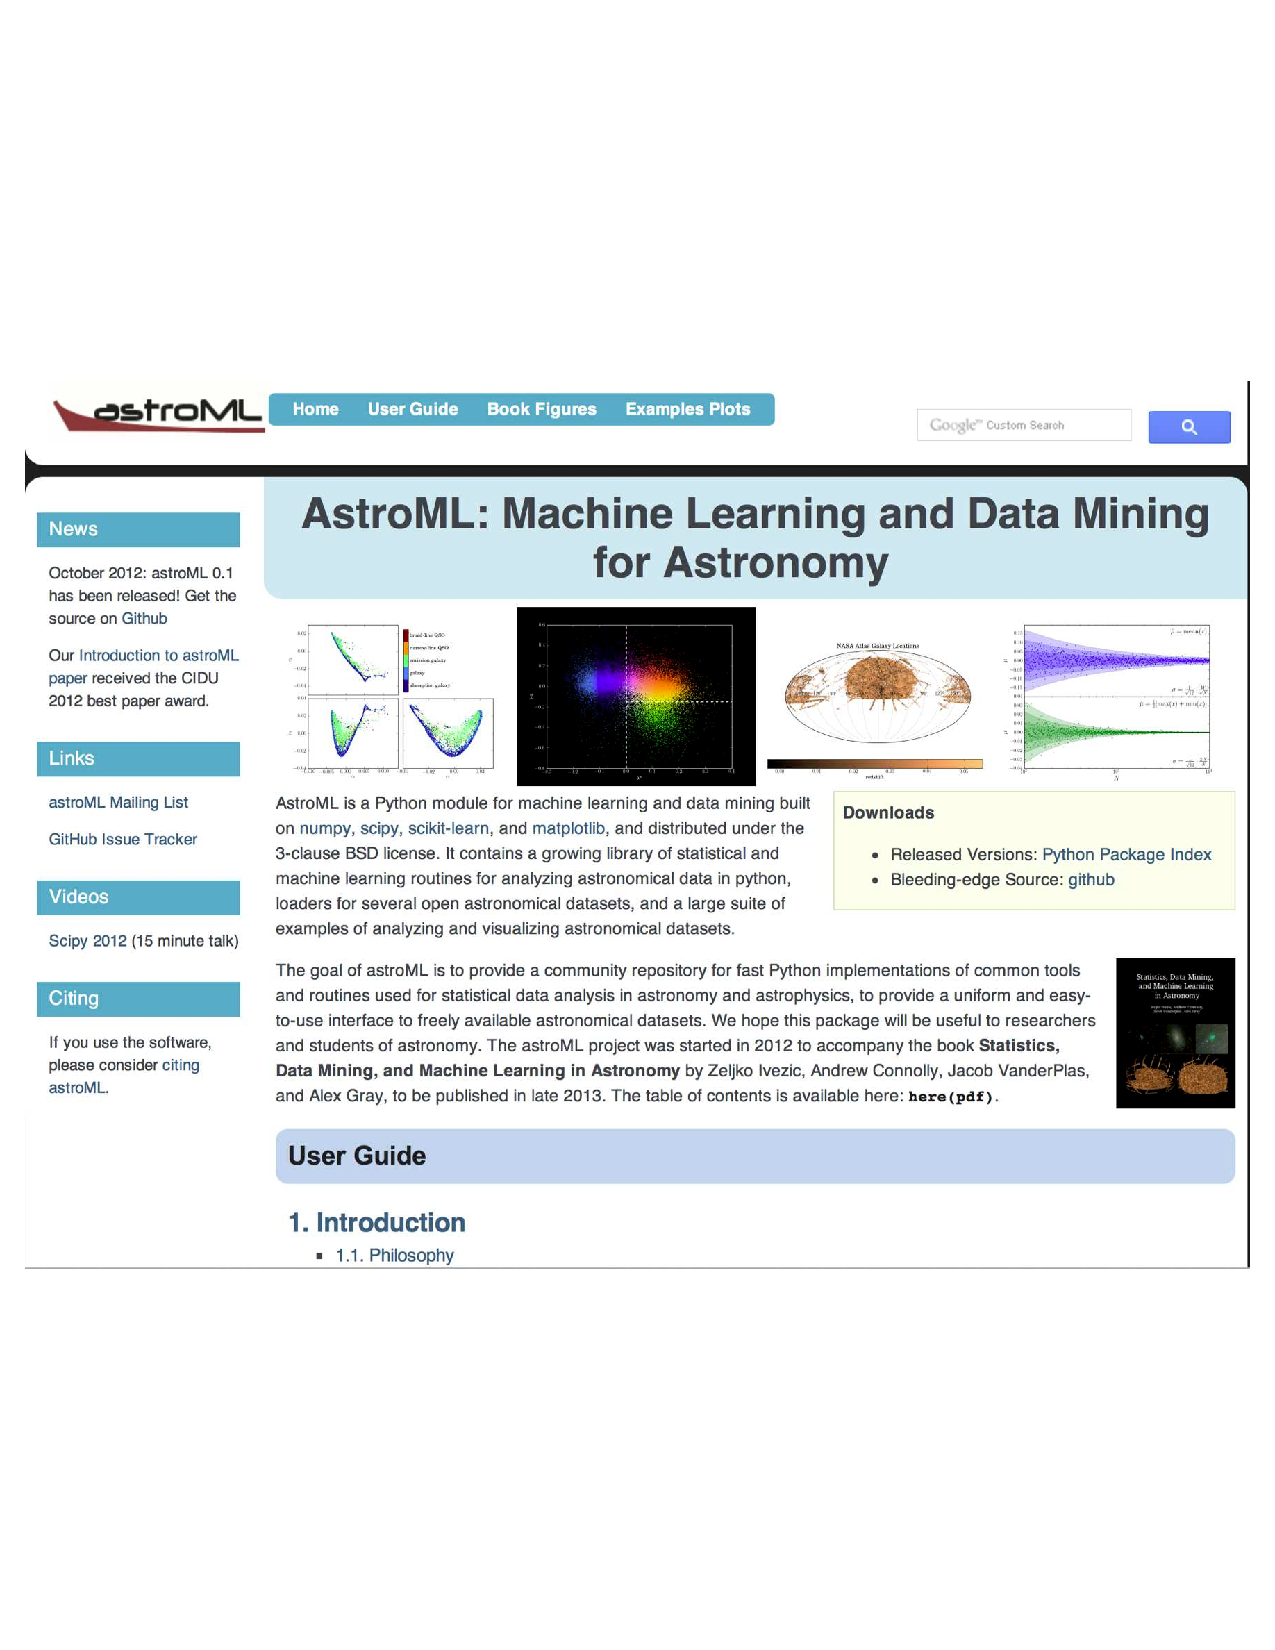
\includegraphics[width=1.02\hsize,clip]{astroML.pdf}
\vskip -2.0in
\caption{We will leverage all the modern Python tools available in {\it astroML} and
other packages, including a large number of practical data-intensive exercises developed to
support textbook that will be used with the proposed \astrocl~ course.} 
\label{Fig:astroML}
\end{figure*}


We will leverage all the publicly available modern Python tools. In particular, seminar work will be 
built around the {\it astroML} package (available from http://www.astroml.org) that was developed 
by Co-PIs to support the textbook to be used with the proposed \astrocl course. {\it astroML} is a Python module 
for machine learning and data mining built on {\it numpy}, {\it scipy}, {\it scikit-learn}, and {\it matplotlib}, 
and distributed under the 3-clause BSD license. It contains a growing library of statistical and machine 
learning routines for analyzing astronomical data in Python, loaders for several open astronomical datasets, 
and a large suite of examples of analyzing and visualizing astronomical datasets (there are close to two 
hundred examples of machine learning and visualization in the code library that supports the textbook 
alone). In addition to  {\it astroML} package, we will expose students to several other popular and widely
used toolkits (e.g. PyMC for Markov chain Monte Carlo methods, and HealPy for spherical coordinates 
and spherical harmonic transformations). 

As an example of methods and exercises available in  {\it astroML}, we single out methods 
for reducing data dimensionality. Many astronomical analyses must address the question of the 
complexity as well as size of the data set. Dimensionality reduction methods address the
complexity issue  by finding the directions within a multivariate data set that contain most 
of the information. Classical approaches for identifying the principal dimensions include
principal component analysis (PCA), independent component analysis (ICA), and non-negative 
matrix factorization (NMF). These methods are implemented in   {\it astroML}, with a user-friendly 
interface and adequate documentation (see Figure~\ref{Fig:astroML}). Furthermore, {\it astroML} also 
includes easy-to-use code to automatically access and download spectra collected by the Sloan Digital 
Sky Survey (currently a ``gold standard'' for modern astronomical surveys and big data sets; see sdss.org). 
Therefore, an undergraduate student will not only be exposed to modern statistical methods
and a cutting-edge astronomical data set, but will be empowered to actually apply these methods 
to a real complex and massive data set.  The result of this exercise is shown in Figure~\ref{Fig:astroML2}. 
With such a positive experience, it is very likely that students would not have difficulties applying 
the same methods and tools later to scientifically unrelated but mathematically similar problems.  


\begin{figure*}[!t]
\vskip -1.8in
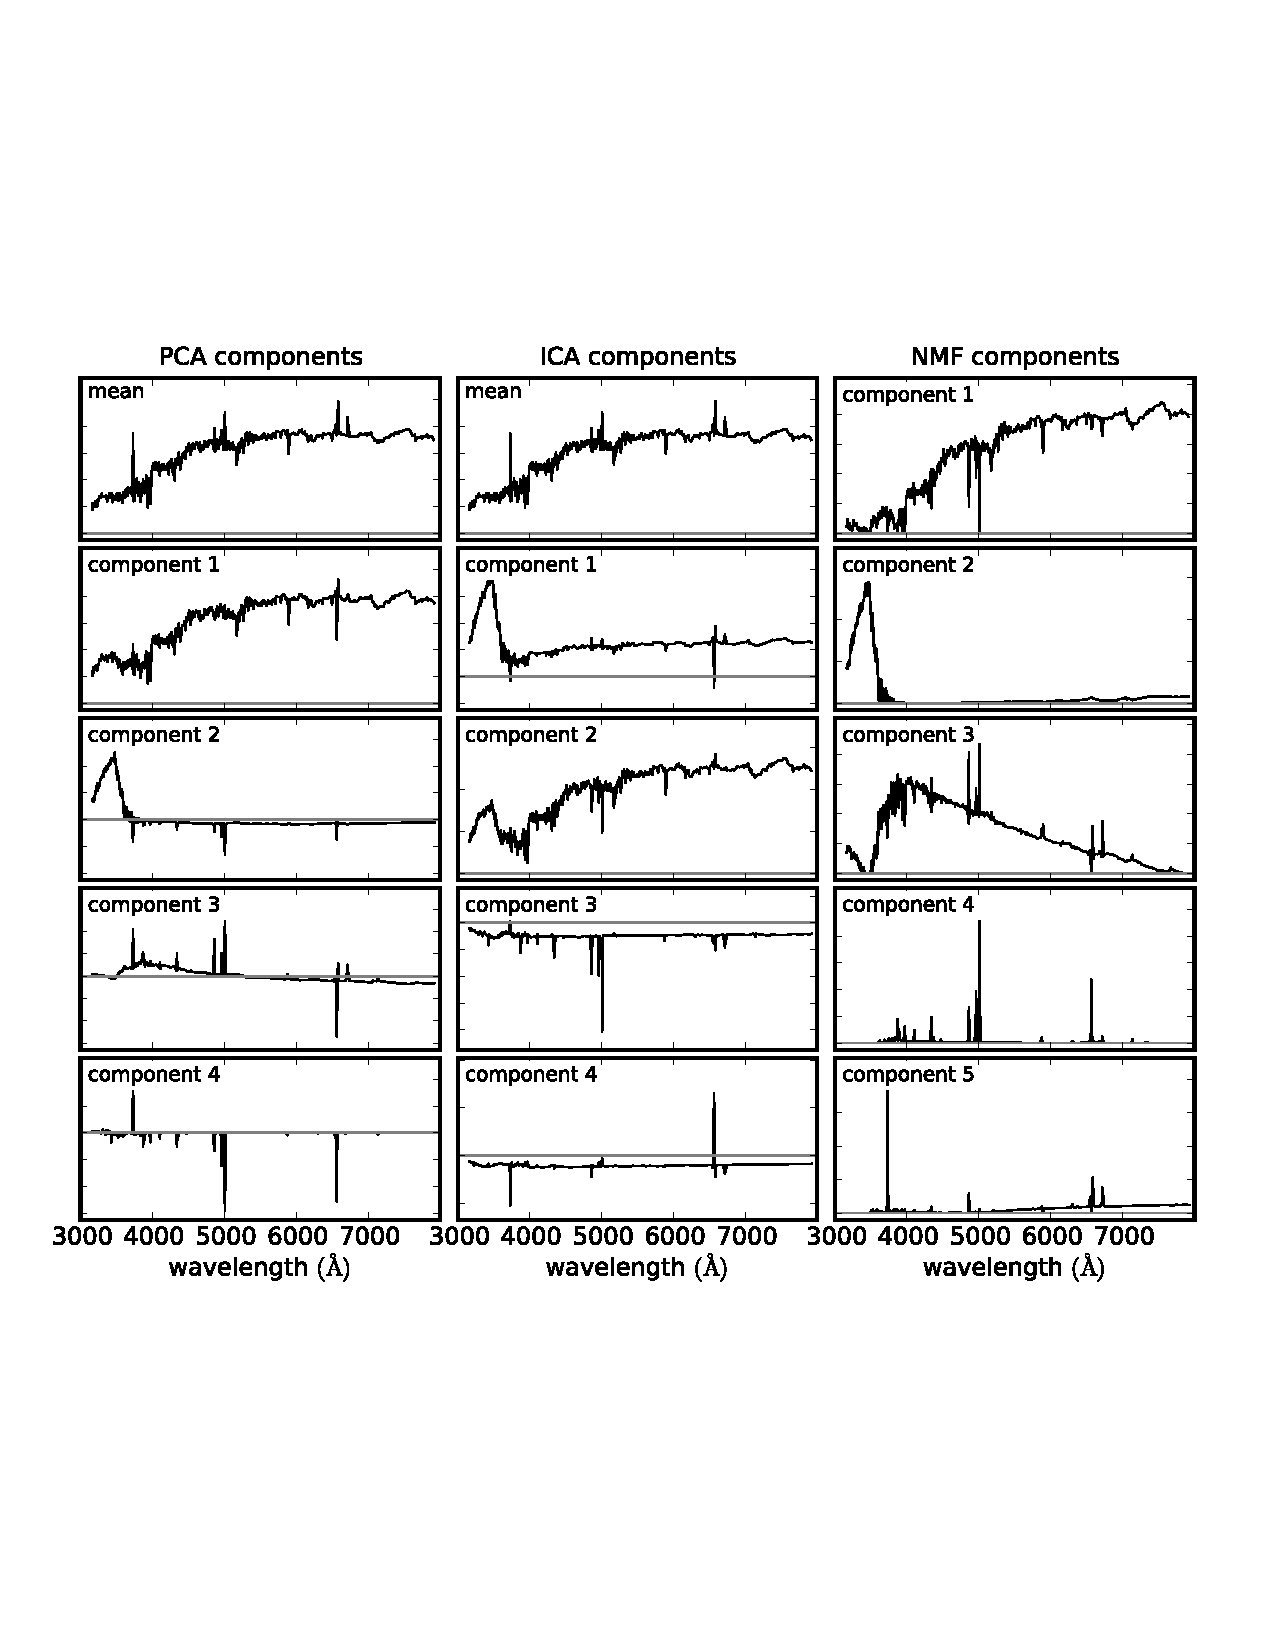
\includegraphics[width=1.02\hsize,clip]{astroML2.pdf}
\vskip -2.0in
\caption{An example of sophisticated tools available in {\it astroML} and exercises that will be
used in practical seminar work. The figure shows a comparison of the decomposition of SDSS 
spectra using PCA (left panel), ICA (middle panel) and NMF (right panel). The rank of the component
increases from top to bottom. For the ICA and PCA the first component is the mean spectrum (NMF 
does not require mean subtraction). All of these techniques isolate a common set of spectral features 
(identifying features associated with the continuum and line emission). The ordering of the spectral 
components is technique dependent. The SDSS spectroscopic database contains over a million
such spectra.} 
\label{Fig:astroML2}
\end{figure*}


\subsection{What we are building on?}
\label{sec:precursors}

\meila~ has extensive previous experience teaching computational
statistics courses at all levels. She developed the
course ``Probability and Statistics for Computer Science'' an
introductory course aimed at computer science majors, complete with exercises and demos in Matlab, revised the Statistical Computing graduate course sequence, later developed the Statistical Learning graduate sequence and led, with prof. Emily Fox, 
the effort to introduce the Machine Learning/Big Data PhD track in the Statistics department. 

\comment{
 under the same
course number \statcl. This has been taught for 11 years at full
enrollment (50 students). From it, what can be transferred to teaching
computing and algorithms to young statisticians? The power of hands on
experience with data, through programs one understands, the
combination of algorithmics and statistics that comes into play for
large, high-dimensional data sets \mmp{clean this up}}

%ZI, AC, JVdP


\meila\ and Connoly co-taught an extremely well received course at CMU
in 1999-2000, ``Computational Statistics of Multi-Dimensional
Scientific Databases'', which reunited students from Statistics,
Computer Science and Astronomy, as well as faculty from these
departments.

The Statistics department runs a {\em Virtual computer lab} that will
be used by \statcl~ students in their quiz sessions and assignments.
%The clusters {\tt newton1,2}, consisting of 8, respectively 2 high memory nodes, 
The high-memory computer clusters, 
accquired from a UW Student Technology Grant, will serve as
basis for the graduate student research. 
% \mmp{shall i buy more nodes??}

The \astroml~ book and web site (see Section \ref{sec:Python}) will provide the starting 
point for the new courses' software and data infrastructure.


\comment{
(Recently, starting 2011, CSE created their own introduction to
probability and statistics, {\sc CSE 312}. Thus it is clear that
\statcl~ can not serve its original purpose and audience.)
\mmp{keep this?}
Therefore, in Spring 2013, the PI \meila with Hoyt Koepke, revised the
course, having in mind that \bit
\item the audience was now literate in statistics and probability
\item the course could now be opened to a larger audience 
\eit
I opted to replace the introductory material with more advanced topics, and for these I chose a set of basic machine learning topics. I also introduced more substantial data analysis assignments. These changes were implemented by Hoyt Kopke, who taught the class. The course web page is at {\tt }. The student feedback to this pilot experiment was very encouraging. \mmp{specifics: how many students, what depts, they liked being made to learn Python, loved the projects too, level was demanding}
}


\comment{OTHER USEFUL INFO
\item These courses fit very well with the original goal and mission of the  ACMS program. 
\item Crosscultural diversity: these classes can also serve science and CSE majors as well as other quantitatively able students across the UW.

{\bf Links}\\
 \statcl Spring 2013 web site {\tt http://www.stat.washington.edu/courses/stat391/spring13/}\\
\astroml~ textbook web site {\tt http://www.amazon.com/Data-Mining-Machine-Learning-Astronomy/dp/0691151695}\\



AMATH 481 Scientific Computing (5)
Project-oriented computational approach to solving problems arising in the physical/engineering sciences, finance/economics, medical, social, and biological sciences. Problems requiring use of advanced MATLAB routines and toolboxes. Covers graphical techniques for data presentation and communication of scientific results. Prerequisite: AMATH 301; either AMATH 351 or MATH 307; either AMATH 352 or MATH 308. Offered: A. 

AMATH 482
Exploratory and objective data analysis methods applied to the physical, engineering, and biological sciences. Brief review of statistical methods and their computational implementation for studying time series analysis, spectral analysis, filtering methods, principal component analysis, orthogonal mode decomposition, and image processing and compression. Prerequisite: AMATH 301; either AMATH 352 or MATH 308. Offered: W.

AMATH 483 High-Performance Scientific Computing (5)
Introduction to hardware, software, and programming for large-scale scientific computing. Overview of multicore, cluster, and supercomputer architectures; procedure and object oriented languages; parallel computing paradigms and languages; graphics and visualization of large data sets; validation and verification; and scientific software development. Prerequisite: either CSE 142 or AMATH 301. Offered: Sp. 

}